%\documentclass{beamer}
%\usetheme{Pittsburgh}
\documentclass{scrartcl}

\usepackage[utf8]{inputenc}
\usepackage{default}
\usepackage[procnames]{listings}
\usepackage{graphicx}
\usepackage{adjustbox}
%\usepackage[toc,page]{appendix}
\usepackage{caption}
\usepackage{hyperref}
\usepackage{color}
%\usepackage{csvsimple}
\usepackage{float}
%\usepackage[T1]{fontenc}



%Bibliogrpahy?
%\usepackage{bibentry}
%\nobibliography*
%\bibentry{ }


%Python
\definecolor{keywords}{RGB}{255,0,90}
\definecolor{comments}{RGB}{0,0,113}
\definecolor{red}{RGB}{160,0,0}
\definecolor{green}{RGB}{0,150,0}
\lstset{language=Python,
    basicstyle=\ttfamily\scriptsize,
    keywordstyle=\color{keywords},
    commentstyle=\color{comments},
    stringstyle=\color{red},
    identifierstyle=\color{green},
    breaklines = true,
    columns=fullflexible,
    %Numbering and tabs
    %numbers=left,
    %numberstyle=\tiny\color{gray},
    %stepnumber=2,
    %numbersep=1em,
    tabsize=4,
    showspaces=false,
    showstringspaces=false}

\begin{document}

\title{Learning and Adaptivity}
\subtitle{Final Report}
\author{
  \href{daiem.ali@smail.inf.h-brs.de}{Ali, Daiem}: \href{https://github.com/daiemna}{github.com/daiemna}\\
  \href{christophe.quignon@smail.inf.h-brs.de}{Quignon, Christophe}:\href{https://github.com/ChrisQuignon}{github.com/ChrisQuignon}
  %Familyname, Name
}
\date{\today}


\maketitle


\begin{abstract}
\textbf{Abstract:}
%TODO we conluded...
\end{abstract}

\section{Problem}
\label{sec:problem}
%TODO: CHECK READ, maybe move to abstract
Heat pumps are a sustainable way to transfer thermal energy into out away from builds to keep a comfortable temperature. But to operate a heating pump is not a trivial task, different building distribute the heat differently and weather with its chaotic nature has a major influence on the temperature flow. In addition, they suffer from a suboptimal efficiency because they often have a bad time delay from sensing to acting. This could be counteracted by predicting future temperatures to overact sensors. efficiency could be increased by predicting energy consumption and delay that to times where energy is cheap. 
Thus we want to predict the behaviour or an energy pump with respect to the weather.


\section{Data}
\label{sec:data}
%TODO: CHECK READ
%what is the problem what is the data wheat is the purpose
The data spans the time between July 2014 to February 2015, with a total of 242 days.

\paragraph{Weather data:}
The regional weather is from the official recordings of the "Deutsche Wetterdienst" (German weather service) and contains:

\begin{itemize}
\item Temperature in $^\circ C$
\item Relative air humidity in percent
\item Precipitation in mm (1 litre per square meter)
\end{itemize}

\paragraph{Sensor data:}
The Measurements from the systems are:

\begin{itemize}
\item Volumetric flow rate in $m^3 / s$
\item Rate of heat flow in watts
\item Supply temperature in $^\circ C$
\item Return temperature $^\circ C$
\end{itemize}

\paragraph{Accumulated data:}
The Energy in watt hours, calculated per day.

\section{Analysis}
\label{sec:analysis}

\subsection{Correlation}
%TODO
\begin{figure}[H]
  %\raggedleft
  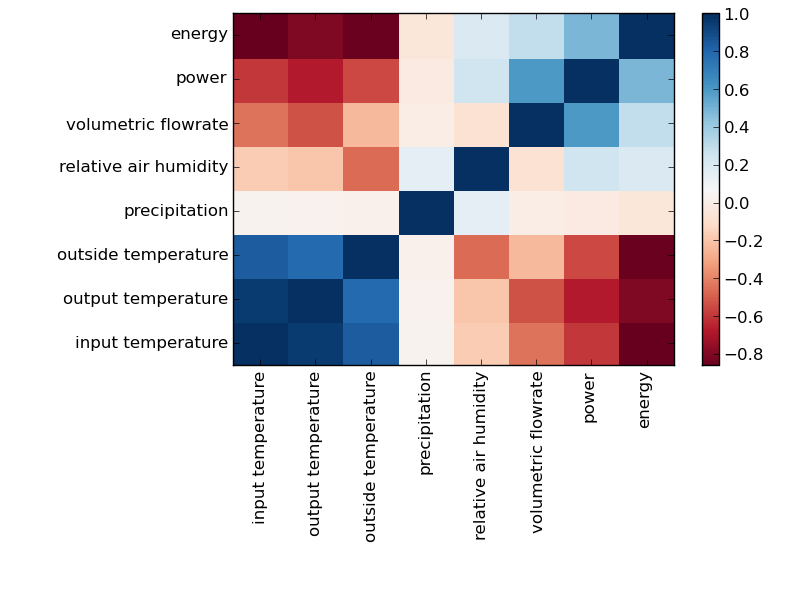
\includegraphics[width=0.6\linewidth]{img/correlation.png}
  \caption{Correlation of the datasets.}
  \label{fig:correlation}
\end{figure}

\subsection{Seasonal decomposition}
%TODO
\begin{figure}[H]
  %\raggedleft
  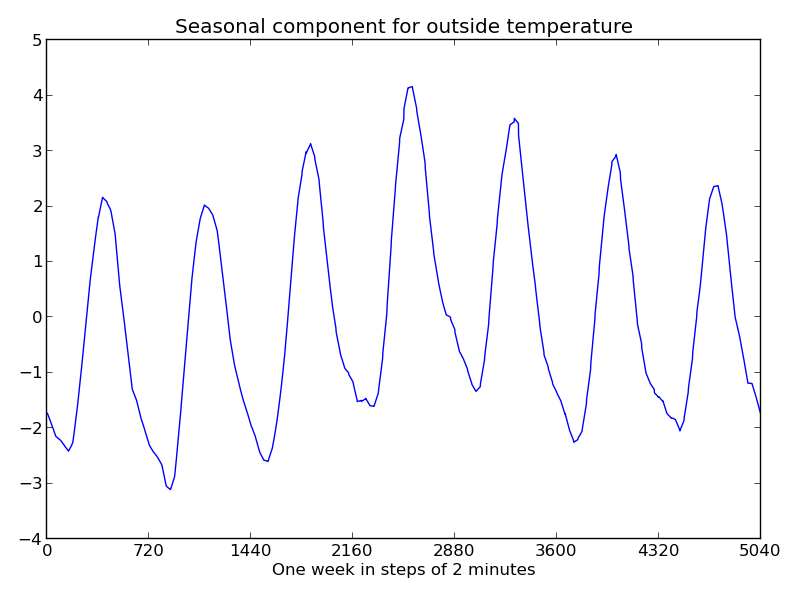
\includegraphics[width=0.6\linewidth]{img/season-outside_temperature.png}
  \caption{Correlation of the datasets.}
  \label{fig:correlation}
\end{figure}


\subsection{Exclusion of precipitation}	
%TODO

\section{Methods}
\label{sec:methods}
%TODO

\subsection{sliding window}
%TODO timeframe analysis

%TODO check read
As suggested in \cite{vafaeipour2014application} the sliding window approach was used to learn how to predict. In this approach the time series is split into windows or frames of input and output. Unlike in regression learning, those windows are shifted. Thus the learning algorithm does not learn the relation of the features at the same time, but their relation in the future. With this approach, it is possible to include all features as an input and select few of them as an output. This can be enhanced further by including predictable features into the input. These three methods are depicted in Figure \ref{fig:slidingwindow}.\\
The random forest implementation we are using however can not handle input with more than one dimension. Thus we flatten the input to one dimension. Since the feature values are typically easily separable, we expect the random forest to recognize this flattening in an early step. We do not include this as an extra information into the trees.
\begin{figure}[H]
  %\raggedleft
  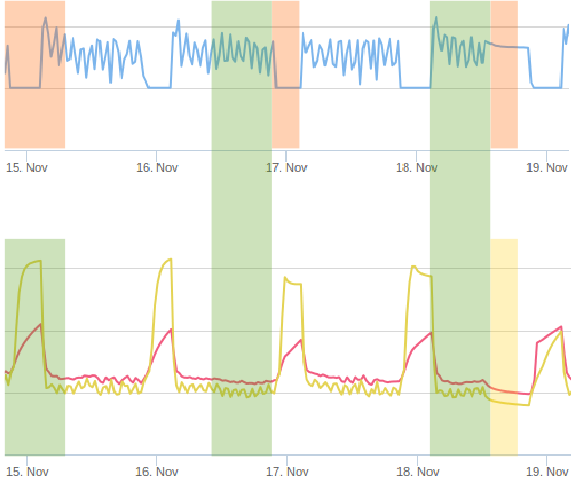
\includegraphics[width=0.6\linewidth]{img/regpred.png}
  \caption{Input(green) and output(red) frames for regression(left), prediction(middle) and enhanced prediction(right).}
  \label{fig:correlation}
\end{figure}

\subsection{gradient boost}
%TODO

\section{Conclusion}
\label{sec:conclusion}
%best result:
%sliding window with DOY
%Prediction output
\begin{figure}[H]
  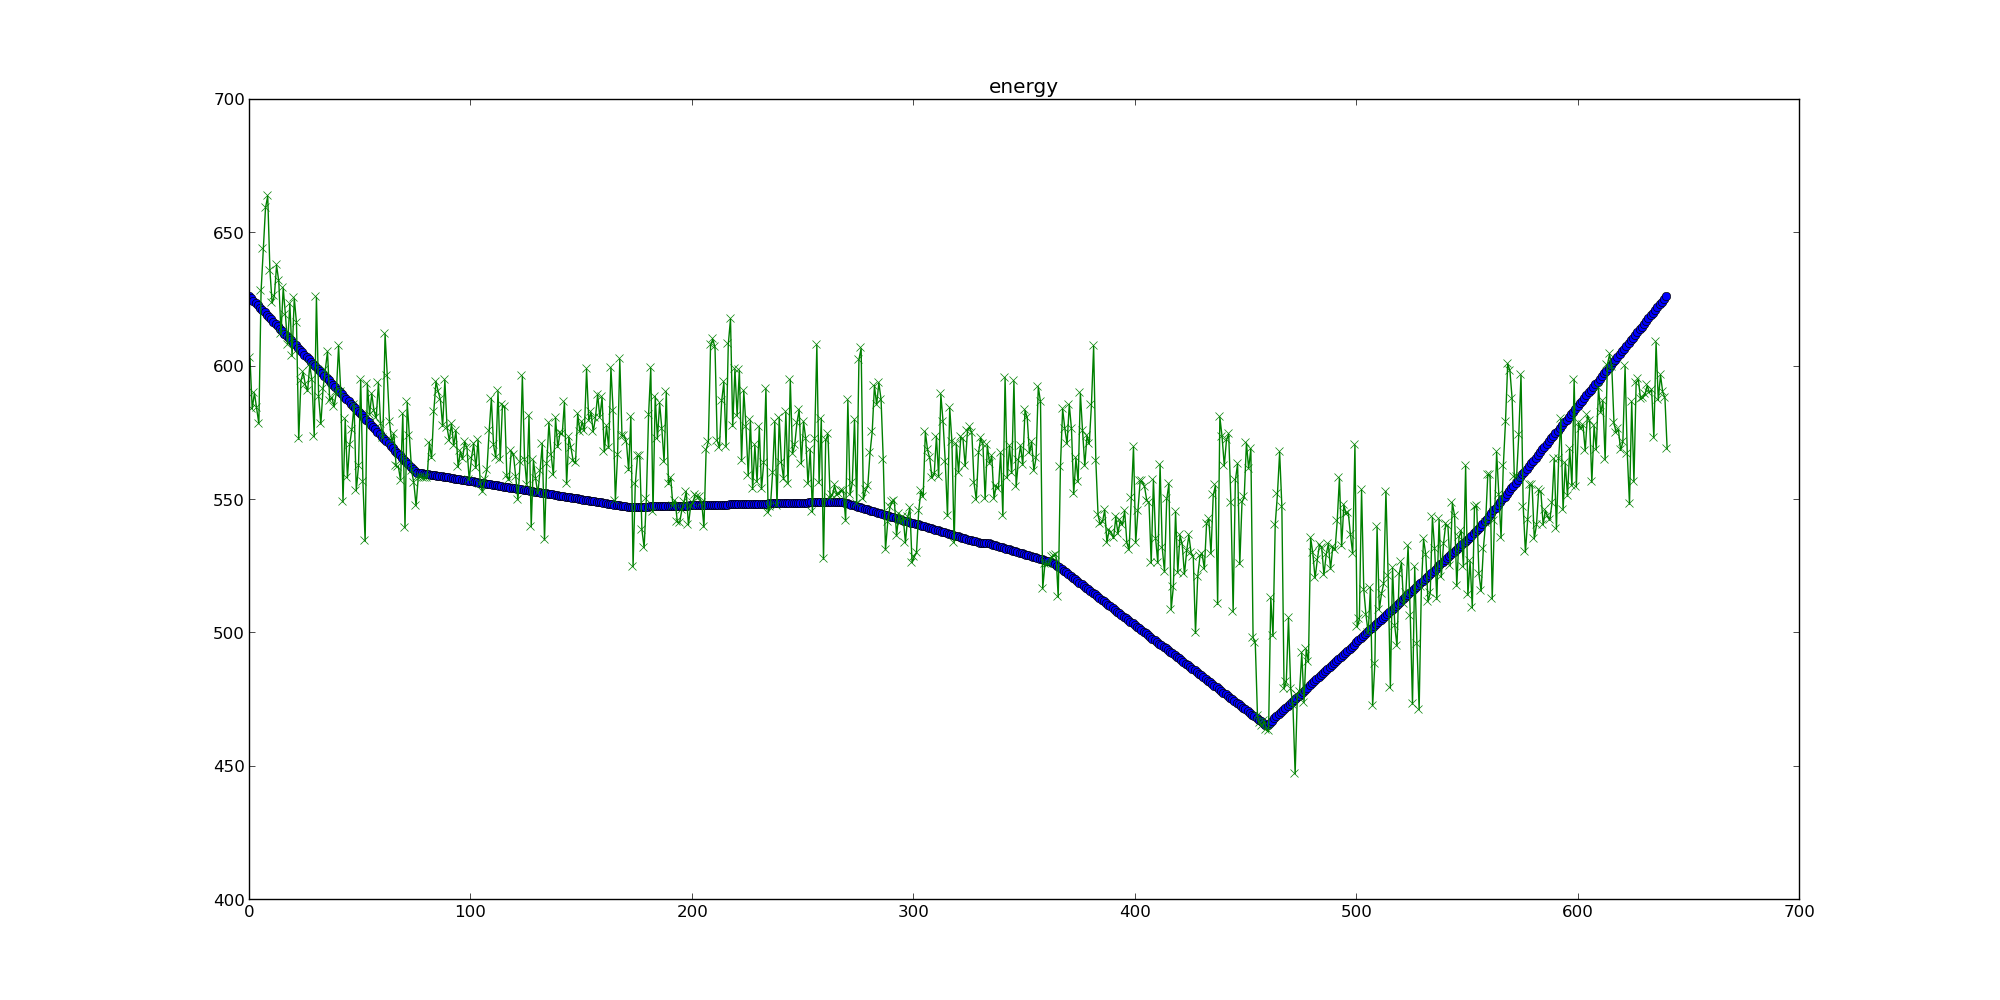
\includegraphics[width=0.6\linewidth]{img/predict-energy-53--0p520.png}
  \caption{Prediction of the energy using the sliding window approach.}
  \label{fig:Prediction}
\end{figure}

%score/error
%application conclusion


%BIBLIOGRPAHY
%TODO: check and fill the bibliography
\bibliographystyle{plain}%amsalpha
\bibliography{bib.bib}
%\bibentry{}

%\begin{appendix}
%\section{}

%\end{appendix}


%COPY AND PASTE FROM HERE

%\begin{enumerate}
% \item
%\end{enumerate}

%\href{link}{text}

%\begin[Language=Python]{lstlisting}
%#PYTHON CODE HERE
%\end{lstlisting}

%\lstinputlisting[language=Python]{	}

%\csvautotabular[separator=semicolon]{data.csv}


%\begin{figure}[H]
%  \centering
%  \includegraphics[width=0.5\linewidth]{../img/	}
%  %\caption{}
%  %\label{fig:}
%\end{figure}
%PUT UNITS ON THE FIGURES

\end{document}
